\let\negmedspace\undefined
\let\negthickspace\undefined
\documentclass[journal]{IEEEtran}
\usepackage[a5paper, margin=10mm, onecolumn]{geometry}
%\usepackage{lmodern} % Ensure lmodern is loaded for pdflatex
\usepackage{tfrupee} % Include tfrupee package

\setlength{\headheight}{1cm} % Set the height of the header box
\setlength{\headsep}{0mm}     % Set the distance between the header box and the top of the text

\usepackage{gvv-book}
\usepackage{gvv}
\usepackage{cite}
\usepackage{amsmath,amssymb,amsfonts,amsthm}
\usepackage{algorithmic}
\usepackage{graphicx}
\usepackage{textcomp}
\usepackage{xcolor}
\usepackage{txfonts}
\usepackage{listings}
\usepackage{enumitem}
\usepackage{mathtools}
\usepackage{gensymb}
\usepackage{comment}
\usepackage[breaklinks=true]{hyperref}
\usepackage{tkz-euclide} 
\usepackage{listings}
% \usepackage{gvv}                                        
\def\inputGnumericTable{}                                 
\usepackage[latin1]{inputenc}                                
\usepackage{color}                                            
\usepackage{array}                                            
\usepackage{longtable}                                       
\usepackage{calc}                                             
\usepackage{multirow}                                         
\usepackage{hhline}                                           
\usepackage{ifthen}                                           
\usepackage{lscape}
\begin{document}

\bibliographystyle{IEEEtran}
\vspace{3cm}

\title{5.2.51}
\author{EE25BTECH11049 - Sai Krishna Bakki}
\maketitle

\subsection*{Question: } 
    Solve the following system of linear equations.
    \begin{align*}
        5x+2y &= 4
    \end{align*}
    \begin{align*}
        7x + 3y &= 5
    \end{align*}

\textbf{Solution}:\\
The equation of line $L_1$ is,
\begin{align}
    \myvec{5 & 2}\vec{x} = 4
\end{align}
The equation of line $L_2$ is,
\begin{align}
    \myvec{7 & 3}\vec{x} = 5
\end{align}

On putting the equations in a matrix, we will get
\begin{align}
    \implies \myvec{5 & 2\\7 & 3}\vec{x} = \myvec{4\\5}
\end{align}
So the augmented matrix is,
\begin{align}
    \augvec{2}{1}{5 & 2 & 4\\7 & 3 & 5}
\end{align}
\begin{align}
    \augvec{2}{1}{5 & 2 & 4\\7 & 3 & 5}s\xleftrightarrow[]{R_2\rightarrow R_2-\frac{7}{5}R_1}\augvec{2}{1}{5 & 2 & 4\\0 & \frac{1}{5} & \frac{-3}{5}}
\end{align}
\begin{align}
    \augvec{2}{1}{5 & 2 & 4\\0 & \frac{1}{5} & \frac{-3}{5}}\xleftrightarrow[]{R_2\rightarrow 5R_2}\augvec{2}{1}{5 & 2 & 4\\0 & 1 &-3}
\end{align}
\begin{align}
   \augvec{2}{1}{5 & 2 & 4\\0 & 1 & -3}\xleftrightarrow[]{R_1\rightarrow R_1-2R_2}\augvec{2}{1}{5 & 0 &10 \\0 & 1 & -3}
\end{align}
\begin{align}
   \augvec{2}{1}{5 & 0 & 10\\0 & 1 & -3}\xleftrightarrow[]{R_1\rightarrow \frac{1}{5}R_1}\augvec{2}{1}{1 & 0 & 2\\0 & 1 & -3}
\end{align}
\begin{align}
    \implies\vec{x} = \myvec{2\\-3}
\end{align}
Therefore the two lines will intersect at \myvec{2\\-3}.

\begin{figure}[H]
    \centering
    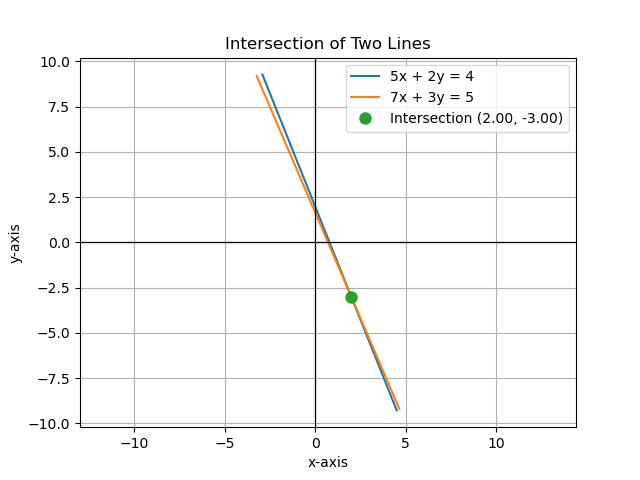
\includegraphics[width=1.0\columnwidth]{figs/Figure_1.png}
    \caption*{}
    \label{fig:}
\end{figure}

\end{document}